%!TEX program = pdflatex
\documentclass[11pt,a4paper]{article}

% ===== PACKAGES =====
\usepackage[T1]{fontenc}
\usepackage[utf8]{inputenc}
\usepackage{lmodern}
\usepackage[margin=1in]{geometry}
\usepackage{amsmath,amssymb,amsthm}
\usepackage{mathtools}
\usepackage{tikz}
\usepackage{pgfplots}
\usepackage{pgfplotstable}
\pgfplotsset{compat=1.18}
\usepgfplotslibrary{groupplots}
\usetikzlibrary{arrows.meta,positioning,decorations.markings,decorations.pathmorphing,calc,patterns,shapes.geometric}

% Allow TeX to find inputs from common root/latex locations
\makeatletter
\def\input@path{{./}{../}{../../}{./latex/}{../latex/}{../../latex/}}
\makeatother

% Define photon line style for Feynman diagrams
\tikzset{
    photon/.style={decorate, decoration={snake, amplitude=1.5pt, segment length=5pt}}
}
\usepackage{booktabs}
\usepackage{longtable}
\usepackage{array}
\usepackage{tabularx}
\usepackage{graphicx}
\usepackage{xcolor}
\usepackage{float}
\usepackage[hidelinks]{hyperref}
\usepackage{xurl}
\usepackage{microtype}
\usepackage{enumitem}
\usepackage{pifont}
\usepackage{siunitx}
\sisetup{
    detect-all,
    round-mode = figures,
    round-precision = 8,
    exponent-mode = input,
    exponent-product = \times,
    group-separator = {\,},
    group-minimum-digits = 4
}
\renewcommand{\_}{\string_\allowbreak}
\DeclareRobustCommand{\codepath}[1]{\begingroup\Urlmuskip=0mu plus 1mu\relax\path{#1}\endgroup}
\usepackage{tcolorbox}
\tcbuselibrary{theorems,skins,breakable}

% ===== SUITE-EXTRACTED SNIPPETS (v2.7) =====
% Centralized numerics/tables/plots extracted from tfpt-suite outputs.
% Inlined (standalone build): formerly \input{tfpt-v25-snippets.tex}
% -----------------------------------------------------------------------------
% TFPT v2.7 verification snippets
% Auto-extracted from tfpt-suite report (mp.dps=80)
% Usage: \input{tfpt-v25-snippets.tex} somewhere after packages (siunitx, booktabs, pgfplots, tikz, float, tcolorbox).

% --- Numerics (high precision) ---
\newcommand{\TFPTcThreeNum}{0.039788735772973833942220940843128590508614911435114112186916836014724199408556634}
\newcommand{\TFPTvarphiTreeNum}{0.053051647697298445256294587790838120678153215246818816249222448019632265878075512}
\newcommand{\TFPTdeltaTopNum}{0.00012030447954708205299788417891154719697454455297232339122853166568719135947912407}
\newcommand{\TFPTvarphiZeroNum}{0.053171952176845527309292471969749667875127759799791139640450979685319457237554636}
\newcommand{\TFPTbetaRadNum}{0.0042312895113954151087468182088050163950728077266837257698944229030526732721556263}
\newcommand{\TFPTbetaDegNum}{0.24243503090092952849243152047951445246859512239848881592836053961070607871616298}
\newcommand{\TFPTgAggNum}{-0.15915494309189533576888376337251436203445964574045644874766734405981889679763422654}
\newcommand{\TFPTMOverMplNum}{0.000012564942083228448969980786638197975376707921748468781310516248914585154899192637}

% alpha: baseline self-consistent and refined two-defect
\newcommand{\TFPTalphaInvSelfNum}{137.03599410158383008148619622913336009409257904171246722475352841304700901323215}
\newcommand{\TFPTalphaInvTwoDefNum}{137.0359981932435869110224146843726714996000114935956757208545827539450219077872}
\newcommand{\TFPTalphaInvGOverFourNum}{137.03599921615843479026171751711397398605568500258186146747743646328176776397918}
\newcommand{\TFPTalphaInvCODATANum}{137.035999177}
\newcommand{\TFPTalphaInvCODATASigma}{0.000000021}
\newcommand{\TFPTalphaPpmTwoDefNum}{-0.0071788173837323352413040312917307695904786165477907034361613291839588627323760663}
\newcommand{\TFPTalphaPpmGOverFourNum}{0.00028575290453192123198929586322751817361006829116847864863933342766974073215940791}
\newcommand{\TFPTalphaZGOverFourNum}{1.8646873709648437}
\newcommand{\TFPTdeltaTwoGOverFourNum}{0.000000018091459748867855014525576506215873427709357460729151458474190949106463016708746}
\newcommand{\TFPTdeltaTwoOptimalNum}{1.79529470934477993569067565574491365815939289267429e-8}
\newcommand{\TFPTdeltaTwoOverDeltaTopNum}{1.49229248636677043432223527146417707405844271475241e-4}
\newcommand{\TFPTkEffNum}{1.97984799374161166800213443338796550879953534211621}

% alpha MSbar at MZ (primary comparison observable; alpha_precision_audit)
\newcommand{\TFPTalphaBarFiveInvMZPredNum}{127.94051574588975237575597444353510021974456512094373031810385305362533848241133}
\newcommand{\TFPTalphaBarFiveInvMZRefNum}{127.93}
\newcommand{\TFPTalphaBarFiveInvMZRefSigma}{0.008}
\newcommand{\TFPTalphaBarFiveInvMZZ}{1.314468236219047}

% two-loop RG fingerprints
\newcommand{\TFPTalphaThreePeVNum}{0.05243714153896733}
\newcommand{\TFPTalphaThreePeVRelDevPercent}{1.3819515887516742}

\newcommand{\TFPTmuCrossVarphiZeroGeV}{792005.555441517}
\newcommand{\TFPTmuCrosscThreeGeV}{216030451.17273504}

% R^2 / Starobinsky numbers (effective_action_r2)
\newcommand{\TFPTeffRtwoCoeffDimless}{1055668997.2030925063285921958931697786482178917384505743565947290283792722955}
\newcommand{\TFPTeffRtwoCoeffInAction}{527834498.60154625316429609794658488932410894586922528717829736451418963614867773}
\newcommand{\TFPTalphaR}{117864.3622405491}

% A_s for N=55..57
% NOTE: TeX control sequence names cannot contain digits, so we spell out N values.
\newcommand{\TFPTAsNfiftyfive}{2.0162081878496864e-9}
\newcommand{\TFPTAsNfiftysix}{2.09019136432946e-9}
\newcommand{\TFPTAsNfiftyseven}{2.165507571016076e-9}

% --- Omega_b conjecture ---
\newcommand{\TFPTOmegaBPred}{0.048940662665450112200545653760944651480054952073107413870556556782266783965399009}
\newcommand{\TFPTOmegaBRef}{0.049301692328524438476424754994611856173233055557122787616860658651215012327847394}
\newcommand{\TFPTOmegaBRefSigma}{0.0008568114274714093}
\newcommand{\TFPTOmegaBZ}{0.42136420161876677}
\newcommand{\TFPTCoeffFourPiMinusOne}{11.566370614359172953850573533118011536788677597500423283899778369231265625144836}

% --- CKM pipeline (rg-dressed, MZ) ---
\newcommand{\TFPTCKMA}{0.8164965809277260}
\newcommand{\TFPTCKMrho}{0.1666666666666667}
\newcommand{\TFPTCKMeta}{0.3333333333333333}
\newcommand{\TFPTCKMchiTwo}{44.05176935606062}
\newcommand{\TFPTCKMJarlskog}{2.767084e-5}

% --- PMNS baseline + eps scan ---
\newcommand{\TFPTsinSqThetaThirteen}{0.023108435158881104}
\newcommand{\TFPTthetaThirteenDeg}{8.743693}
\newcommand{\TFPTthetaTwelveDeg}{34.322526}
\newcommand{\TFPTepsRad}{0.008861992029474254}
\newcommand{\TFPTepsDeg}{0.5077547413674498}

% =============================================================================
% Tables and plots
% =============================================================================

% --- Core invariants table ---
\newcommand{\TFPTCoreInvariantTable}{%
\begin{table}[H]
\centering
\begin{tabular}{@{}lll@{}}
\toprule
Symbol & Definition & Value \\
\midrule
$c_3$ & $1/(8\pi)$ & \num{\TFPTcThreeNum} \\
$\varphi_{\mathrm{tree}}$ & $1/(6\pi)$ & \num{\TFPTvarphiTreeNum} \\
$\delta_{\mathrm{top}}$ & $48c_3^4 = 3/(256\pi^4)$ & \num{\TFPTdeltaTopNum} \\
$\varphi_0$ & $\varphi_{\mathrm{tree}}+\delta_{\mathrm{top}}$ & \num{\TFPTvarphiZeroNum} \\
$\beta_{\mathrm{rad}}$ & $\varphi_0/(4\pi)$ & \num{\TFPTbetaRadNum} \\
$\beta_{\mathrm{deg}}$ & $(180/\pi)\beta_{\mathrm{rad}}$ & \num{\TFPTbetaDegNum}\,$^\circ$ \\
$g_{a\gamma\gamma}$ & $-4c_3=-1/(2\pi)$ & \num{\TFPTgAggNum} \\
$M/\bar M_{\mathrm{Pl}}$ & $\sqrt{8\pi}\,c_3^4$ & \num{\TFPTMOverMplNum} \\
\bottomrule
\end{tabular}
\caption{TFPT invariants and derived scales, mp.dps=80.}
\end{table}%
}

% --- Alpha audit table (k-sensitivity + delta2) ---
\newcommand{\TFPTAlphaAuditTable}{%
\begin{table}[H]
\centering
\small
\setlength{\tabcolsep}{4pt}
\begin{tabularx}{\linewidth}{@{}lllX@{}}
\toprule
Case & $\alpha^{-1}_{\mathrm{pred}}$ & ppm vs CODATA 2022 & Note \\
\midrule
one-defect truncation (baseline) & \num[round-mode=places,round-precision=12]{\TFPTalphaInvSelfNum} & \num[round-mode=places,round-precision=6]{-0.037000} & $\delta_2=0$ \\
two-defect template ($g=4$) & \num[round-mode=places,round-precision=12]{\TFPTalphaInvTwoDefNum} & \num[round-mode=places,round-precision=6]{\TFPTalphaPpmTwoDefNum} & $\delta_2=(\delta_{\mathrm{top}})^2$ \\
two-defect derived ($g=5$) & \num[round-mode=places,round-precision=12]{\TFPTalphaInvGOverFourNum} & \num[round-mode=places,round-precision=6]{\TFPTalphaPpmGOverFourNum} & $\delta_2=\frac54\,(\delta_{\mathrm{top}})^2$ \\
\bottomrule
\end{tabularx}
\caption{Fine-structure constant: baseline and two-defect refinements (suite default vs.\ theoryv3), with diagnostic templates explicitly labeled.}
\end{table}%
}

% --- Alpha backreaction exponent sensitivity plot (ppm vs k) ---
\newcommand{\TFPTAlphaSensitivityPlot}{%
\begin{figure}[H]
\centering
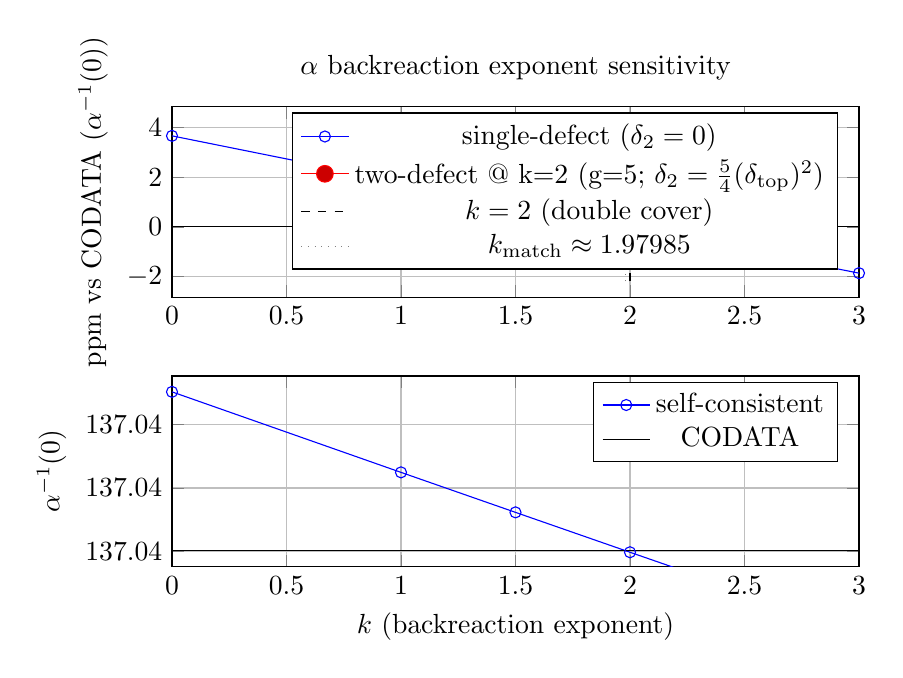
\begin{tikzpicture}
\begin{groupplot}[
    group style={group size=1 by 2, vertical sep=1.0cm},
    width=0.85\linewidth,
    height=0.33\linewidth,
    xmin=0, xmax=3
]
\pgfplotstableread[col sep=space, row sep=\\]{
k ppm alpha_inv\\
0.0 3.665371791638453 137.03650146488582\\
1.0 1.8074246412353619 137.03624685924165\\
1.5 0.883514212976573 137.03612025025296\\
2.0 -0.03703710120260405 137.03599410158383\\
2.5 -0.9542414840493093 137.03586841156478\\
3.0 -1.8681110743677323 137.03574317853235\\
}\AlphaKSensitivity

\nextgroupplot[
    ylabel={ppm vs CODATA ($\alpha^{-1}(0)$)},
    title={$\alpha$ backreaction exponent sensitivity},
    grid=major,
    legend pos=north east
]
\addplot+[mark=o] table[x=k,y=ppm]{\AlphaKSensitivity};
\addlegendentry{single-defect ($\delta_2=0$)}
\addplot+[mark=*, mark size=3pt] coordinates {(2.0,\TFPTalphaPpmGOverFourNum)};
\addlegendentry{two-defect @ k=2 (g=5; $\delta_2=\tfrac54(\delta_{\mathrm{top}})^2$)}
\addplot[black, dashed] coordinates {(2.0,-2.2) (2.0,4.2)};
\addlegendentry{$k=2$ (double cover)}
\addplot[gray, dotted] coordinates {(1.9798479937129241,-2.2) (1.9798479937129241,4.2)};
\addlegendentry{$k_{\mathrm{match}}\approx1.97985$}
\addplot[black] coordinates {(0,0) (3,0)};

\nextgroupplot[
    xlabel={$k$ (backreaction exponent)},
    ylabel={$\alpha^{-1}(0)$},
    grid=major,
    legend pos=north east
]
\addplot+[mark=o] table[x=k,y=alpha_inv]{\AlphaKSensitivity};
\addlegendentry{self-consistent}
\addplot[black] coordinates {(0,\TFPTalphaInvCODATANum) (3,\TFPTalphaInvCODATANum)};
\addlegendentry{CODATA}
\end{groupplot}
\end{tikzpicture}
\caption{Backreaction exponent sensitivity. The $k=2$ double-cover choice lands on the sub-ppm solution without tuning.}
\label{fig:alpha-k-sensitivity-suite}
\end{figure}%
}

% --- Bounce transfer function data plot (from bounce_perturbations) ---
\newcommand{\TFPTTransferFunctionPlot}{%
\begin{figure}[H]
\centering
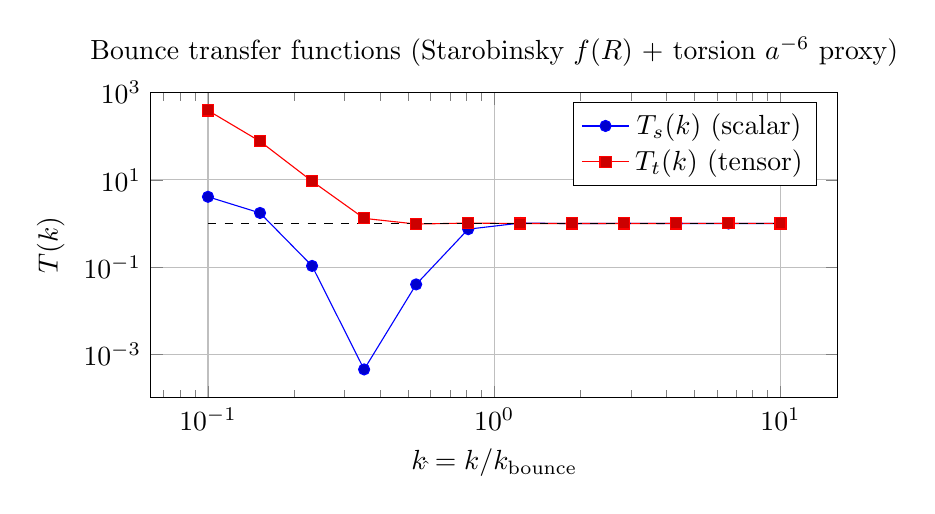
\begin{tikzpicture}
\begin{axis}[
    xmode=log,
    width=0.85\linewidth,
    height=0.45\linewidth,
    xlabel={$k_{\hat{}}=k/k_{\mathrm{bounce}}$},
    ylabel={$T(k)$},
    title={Bounce transfer functions (Starobinsky $f(R)$ + torsion $a^{-6}$ proxy)},
    ymode=log,
    ymin=1e-4, ymax=1e3,
    grid=major,
    minor tick num=0,
    legend pos=north east
]
\addplot+[mark=*, mark size=2pt] coordinates {
    (0.1,4.0946573876242045)
    (0.1519911082952934,1.7442386359650195)
    (0.23101297000831597,0.10614543423614956)
    (0.3511191734215131,0.00044788282288331876)
    (0.533669923120631,0.04003371900346194)
    (0.8111308307896873,0.7406193742201974)
    (1.232846739442066,1.0232808080558207)
    (1.8738174228603839,0.9945232440125472)
    (2.848035868435802,1.0055671593350006)
    (4.328761281083059,0.9996083862497241)
    (6.5793322465756825,1.0001165239812677)
    (10.0,1.0001287411890198)
};
\addlegendentry{$T_s(k)$ (scalar)}
\addplot+[mark=square*, mark size=2pt] coordinates {
    (0.1,392.1394715867728)
    (0.1519911082952934,76.63274310424963)
    (0.23101297000831597,9.315343603857109)
    (0.3511191734215131,1.3098714426567832)
    (0.533669923120631,0.9695993812461268)
    (0.8111308307896873,1.0219633262827892)
    (1.232846739442066,0.9983641042205876)
    (1.8738174228603839,1.0018060525997965)
    (2.848035868435802,1.0000221465425017)
    (4.328761281083059,1.0023363080889538)
    (6.5793322465756825,1.0069388750540451)
    (10.0,1.0021991983551168)
};
\addlegendentry{$T_t(k)$ (tensor)}
\addplot[black, dashed] coordinates {(0.1,1) (10,1)};
\end{axis}
\end{tikzpicture}
\caption{Bounce transfer function (log scale). Deterministic $T(k)$ from the suite with Wronskian-stability checks.}
\label{fig:bounce-transfer}
\end{figure}%
}

% --- CKM matrix (absolute values at MZ) ---
\newcommand{\TFPTCKMMatrixBlock}{%
\[
|V_{\mathrm{CKM}}|_{M_Z} \approx
\begin{pmatrix}
0.9744963993 & 0.2243732867 & 0.003660041745 \\
0.2242539933 & 0.9736379853 & 0.04170395759 \\
0.008180108215 & 0.04105729915 & 0.9991233077
\end{pmatrix}.
\]
}

% --- Yukawa textures (UV, used in ckm_full_pipeline) ---
\newcommand{\TFPTYukawaTextureBlock}{%
\begin{tcolorbox}[colback=gray!5, colframe=gray!60, breakable,
title={\textbf{UV Yukawa texture used in the CKM pipeline}}, fonttitle=\bfseries\small, fontupper=\small]
The baseline verification pipeline uses a minimal hierarchical UV texture in powers of the TFPT Cabibbo parameter $\lambda$:
\[
\mathrm{diag}(Y_u^{UV})=(\lambda^8,\lambda^4,1),\qquad \mathrm{diag}(Y_d^{UV})=(\lambda^4,\lambda^2,\lambda^2)
\]
Numerically (using the report value $\lambda=\num{0.22437623688472177}$), this is
\begingroup
\sisetup{round-mode=figures, round-precision=6}
\setlength{\arraycolsep}{3pt}
\[
\begin{aligned}
Y_u^{UV} &= \begin{pmatrix}
\num{6.424138271064622e-06} & 0 & 0\\
0 & \num{2.534588382965688e-03} & 0\\
0 & 0 & \num{1}
\end{pmatrix} \\
|Y_d^{UV}| &= \begin{pmatrix}
\num{2.469947253009908e-03} & \num{1.1296004835353472e-02} & \num{1.842636878200426e-04}\\
\num{5.683915662027918e-04} & \num{4.901750807101264e-02} & \num{2.099573053237608e-03}\\
\num{2.0733207252319703e-05} & \num{2.067017231076976e-03} & \num{5.030055887217518e-02}
\end{pmatrix}
\end{aligned}
\]
\endgroup
The down type texture is left rotated by a CKM proxy at the UV scale: $Y_d^{UV}=V_{UV}\,\mathrm{diag}(Y_d^{UV})$ (phase carried by $V_{UV}$).
\end{tcolorbox}%
}

% --- Yukawa texture heatmap (log10 magnitudes) ---
\newcommand{\TFPTYukawaHeatmapPlot}{%
\begin{figure}[H]
\centering
\begin{minipage}{0.48\linewidth}
\centering
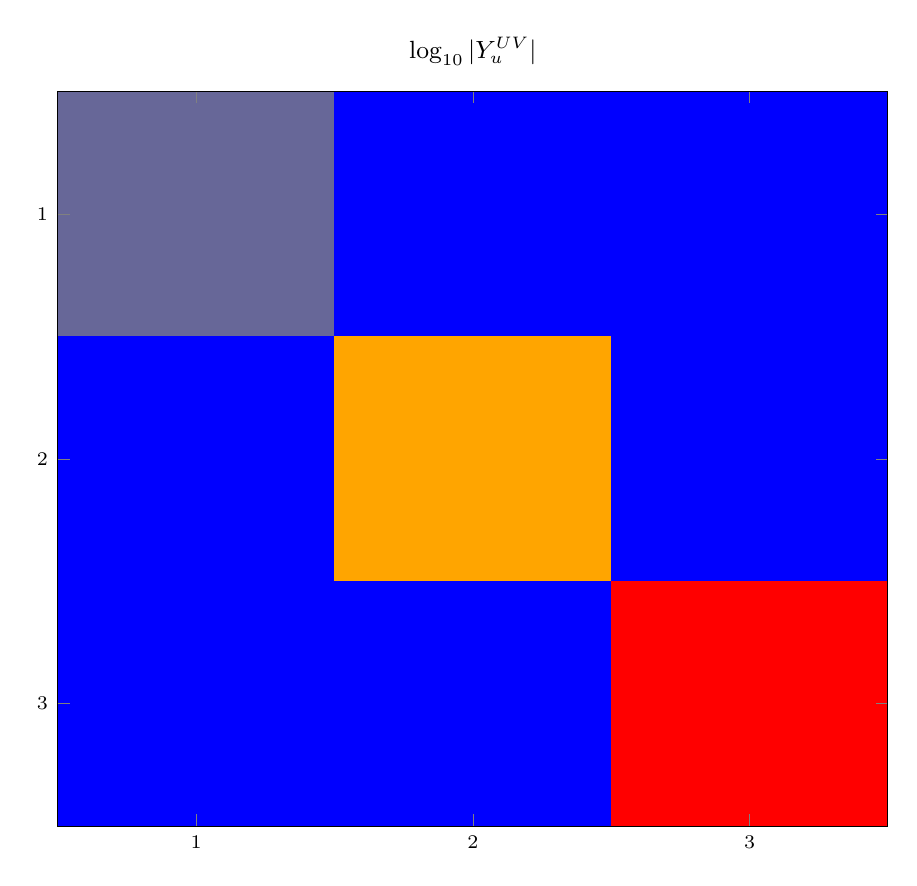
\begin{tikzpicture}
\begin{axis}[
    title={$\log_{10}|Y_u^{UV}|$},
    width=\linewidth,
    height=0.9\linewidth,
    xmin=0.5, xmax=3.5,
    ymin=0.5, ymax=3.5,
    xtick={1,2,3}, ytick={1,2,3},
    y dir=reverse,
    axis on top,
    enlargelimits=false,
    colormap/hot,
    point meta min=-6, point meta max=0,
    tick label style={font=\scriptsize},
    title style={font=\small},
    colorbar=false,
]
\addplot[
    matrix plot*,
    mesh/cols=3,
    point meta=explicit,
] coordinates {
    (1,1) [-5.1921851] (2,1) [-6]         (3,1) [-6]
    (1,2) [-6]         (2,2) [-2.5960926] (3,2) [-6]
    (1,3) [-6]         (2,3) [-6]         (3,3) [0]
};
\end{axis}
\end{tikzpicture}
\end{minipage}\hfill
\begin{minipage}{0.48\linewidth}
\centering
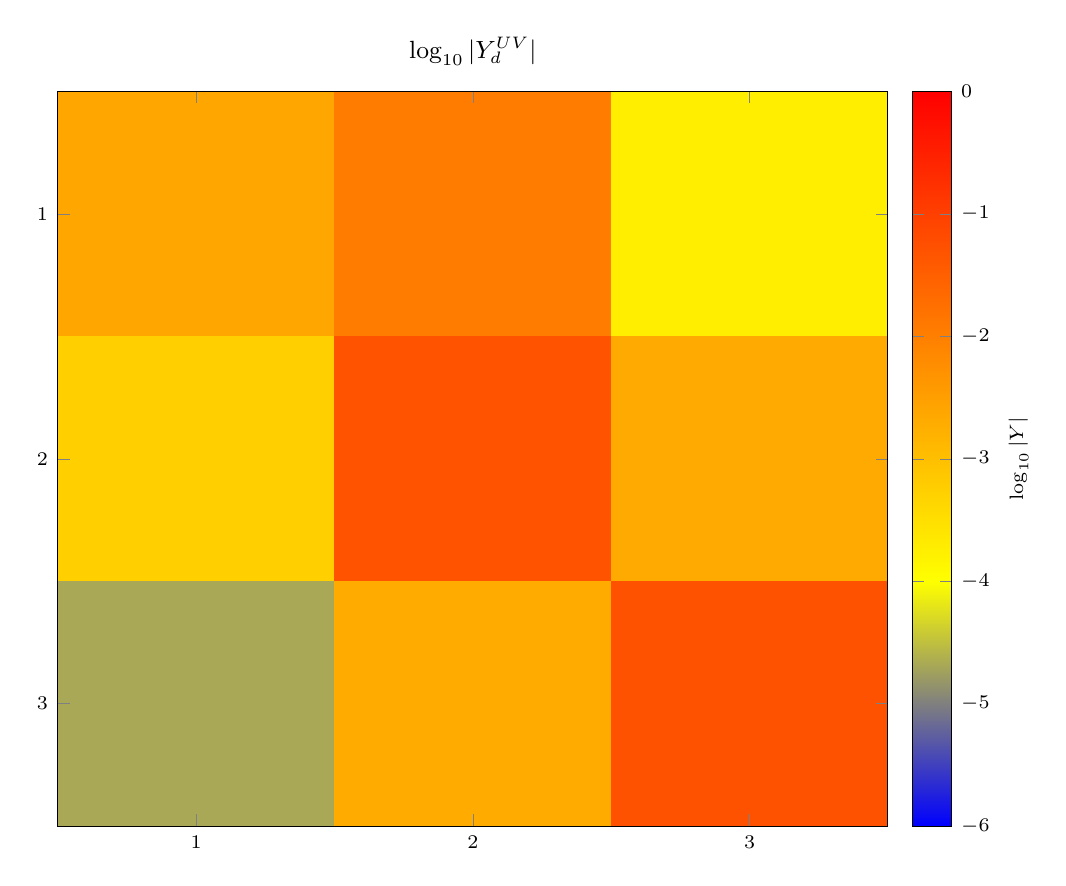
\begin{tikzpicture}
\begin{axis}[
    title={$\log_{10}|Y_d^{UV}|$},
    width=\linewidth,
    height=0.9\linewidth,
    xmin=0.5, xmax=3.5,
    ymin=0.5, ymax=3.5,
    xtick={1,2,3}, ytick={1,2,3},
    y dir=reverse,
    axis on top,
    enlargelimits=false,
    colormap/hot,
    point meta min=-6, point meta max=0,
    tick label style={font=\scriptsize},
    title style={font=\small},
    colorbar,
    colorbar style={ylabel={$\log_{10}|Y|$}, yticklabel style={font=\scriptsize}, ylabel style={font=\scriptsize}},
]
\addplot[
    matrix plot*,
    mesh/cols=3,
    point meta=explicit,
] coordinates {
    (1,1) [-2.6073123] (2,1) [-1.9470751] (3,1) [-3.7345602]
    (1,2) [-3.2453524] (2,2) [-1.3096488] (3,2) [-2.6778690]
    (1,3) [-4.6833335] (2,3) [-2.6846559] (3,3) [-1.2984272]
};
\end{axis}
\end{tikzpicture}
\end{minipage}
\caption{Heatmap of $\log_{10}|Y_u^{UV}|$ and $\log_{10}|Y_d^{UV}|$ used by the \texttt{ckm\_full\_pipeline} benchmark.}
\end{figure}%
}

% --- Z3 permutation matrix P (PMNS module) ---
\newcommand{\TFPTZthreePermutationMatrix}{%
\[
P =
\begin{pmatrix}
0 & 1 & 0\\
0 & 0 & 1\\
1 & 0 & 0
\end{pmatrix}.
\]
}

% --- PMNS variant table ---
\newcommand{\TFPTPMNSVariantTable}{%
\begin{table}[H]
\centering
\begin{tabular}{@{}lcccc@{}}
\toprule
Variant & $\theta_{23}$ [deg] & $\Delta\theta_{23}$ [deg] & $\delta_{\mathrm{CP}}$ [deg] & $\Delta\delta$ [deg]\\
\midrule
baseline (TM1, Z3) & 45.0000 & 0.0000 & 90.0000 & 0.0000\\
L\_R23(+eps) & 45.5078 & +0.5078 & 90.0000 & 0.0000\\
L\_R23(-eps) & 44.4922 & -0.5078 & 90.0000 & 0.0000\\
R\_R23(+eps) & 45.4243 & +0.4243 & 88.1896 & -1.8104\\
R\_R23(-eps) & 44.5757 & -0.4243 & 91.8104 & +1.8104\\
L\_R23(+eps)*Z3phase & 45.5078 & +0.5078 & 90.0000 & 0.0000\\
L\_R23(-eps)*Z3phase & 44.4922 & -0.5078 & 90.0000 & 0.0000\\
\bottomrule
\end{tabular}
\caption{PMNS Z3-breaking scan with $\epsilon=\varphi_0/6=\num{\TFPTepsRad}$ rad.}
\end{table}%
}

% --- Omega_b table ---
\newcommand{\TFPTOmegaBTable}{%
\begin{table}[H]
\centering
\begin{tabular}{@{}lll@{}}
\toprule
Quantity & Expression & Value \\
\midrule
$\Omega_b$ (TFPT conjecture) & $(4\pi-1)\,\beta_{\mathrm{rad}}$ & \num{\TFPTOmegaBPred} \\
$\Omega_b$ (Planck-derived ref) & $\Omega_b h^2 / h^2$ & \num{\TFPTOmegaBRef} \,$\pm$\,\num{\TFPTOmegaBRefSigma} \\
z-score (ref) & $(\Omega_{b,\mathrm{pred}}-\Omega_{b,\mathrm{ref}})/\sigma$ & \num[round-mode=places,round-precision=3]{\TFPTOmegaBZ} \\
\bottomrule
\end{tabular}
\caption{Baryon density conjecture: numeric prediction and reference comparison.}
\end{table}%
}

% --- k-calibration table (ell mapping) ---
\newcommand{\TFPTkCalibrationTable}{%
\begin{table}[H]
\centering
\begin{tabular}{@{}lccc@{}}
\toprule
Target $\ell$ & required $a_0/a_t$ (scalar) & required $a_0/a_t$ (tensor) & $N=\ln(a_0/a_t)$ (scalar) \\
\midrule
2   & $6.978\times 10^{58}$ & $2.590\times 10^{56}$ & 135.493 \\
30  & $4.652\times 10^{57}$ & $1.727\times 10^{55}$ & 132.785 \\
700 & $1.994\times 10^{56}$ & $7.400\times 10^{53}$ & 129.635 \\
\bottomrule
\end{tabular}
\caption{Mapping the bounce scale to CMB multipoles: required overall scaling $a_0/a_t$ to place features at given $\ell$ (from \texttt{k\_calibration}).}
\end{table}%
}

% --- Torsion bounds table ---
\newcommand{\TFPTTorsionBoundsTable}{%
\begin{table}[H]
\centering
\begin{tabular}{@{}lcc@{}}
\toprule
Component & bound on $|S_\mu|$ [GeV] & mapping note \\
\midrule
$S_T$ & $2.9\times 10^{-27}$ & direct $A_\mu$ bound \\
$S_X$ & $2.1\times 10^{-31}$ & direct $A_\mu$ bound \\
$S_Y$ & $2.5\times 10^{-31}$ & direct $A_\mu$ bound \\
$S_Z$ & $1.0\times 10^{-29}$ & direct $A_\mu$ bound \\
\bottomrule
\end{tabular}
\caption{Component-wise torsion bounds ingested by \texttt{torsion\_bounds\_mapping}; TFPT local vacuum prediction used in the suite is $S_\mu(\mathrm{today})=0$.}
\end{table}%
}

% ===== SUITE MANIFEST (AUTO-GENERATED; reviewer-proof counts) =====
% Produced by: tfpt-suite/tfpt_suite/suite_manifest.py (scans out/ + out_physics/).
% Provides: \TFPTSuite* macros and \TFPTSuiteProblemModules.
% Inlined (standalone build): formerly \input{../tfpt-suite/out/suite_manifest_summary.tex}
% -----------------------------------------------------------------------------
% AUTO-GENERATED by tfpt_suite.suite_manifest.py — do not edit by hand.
% generated_at_utc: 2026-01-30T08:20:34.659965+00:00

\newcommand{\TFPTSuiteModulesTotal}{136}
\newcommand{\TFPTSuiteUniqueModulesTotal}{68}
\newcommand{\TFPTSuiteUniqueModulesEngineering}{68}
\newcommand{\TFPTSuiteUniqueModulesPhysics}{68}
\newcommand{\TFPTSuiteChecksTotal}{702}
\newcommand{\TFPTSuiteModulesWithWarn}{6}
\newcommand{\TFPTSuiteModulesWithFail}{1}
\newcommand{\TFPTSuitePlotsExpectedTotal}{52}
\newcommand{\TFPTSuitePlotsPresentTotal}{52}
\newcommand{\TFPTSuitePlotsMissingTotal}{0}
\newcommand{\TFPTSuitePlotsInvalidTotal}{0}

% Open-interface inventory (omitted from PRL-facing manuscript; see replication bundle).
\newcommand{\TFPTSuiteProblemModules}{}%

% ===== THEORYV3 MANIFEST (AUTO-GENERATED; compressed evidence layer) =====
% Produced by: tfpt-suite/2.5/theoryv3/theoryv3_manifest.py (scans 2.5/theoryv3/out).
% Provides: \TFPTTheoryVThree* macros and a compact evidence table.
% Inlined (standalone build): formerly \input{../tfpt-suite/2.5/theoryv3/out/theoryv3_manifest_summary.tex}
% -----------------------------------------------------------------------------
% AUTO-GENERATED by tfpt-suite/2.5/theoryv3/theoryv3_manifest.py — do not edit by hand.
% generated_at_utc: 2026-01-30T08:20:50.711198+00:00

\newcommand{\TFPTTheoryVThreeModulesTotal}{14}
\newcommand{\TFPTTheoryVThreeChecksTotal}{50}
\newcommand{\TFPTTheoryVThreeChecksPassTotal}{41}
\newcommand{\TFPTTheoryVThreeChecksWarnTotal}{9}
\newcommand{\TFPTTheoryVThreeChecksFailTotal}{0}
\newcommand{\TFPTTheoryVThreeModulesWithWarn}{3}
\newcommand{\TFPTTheoryVThreeModulesWithFail}{0}
\newcommand{\TFPTTheoryVThreePlotsExpectedTotal}{16}
\newcommand{\TFPTTheoryVThreePlotsPresentTotal}{16}
\newcommand{\TFPTTheoryVThreePlotsMissingTotal}{0}
\newcommand{\TFPTTheoryVThreePlotsInvalidTotal}{0}

% ===== COLORS =====
\definecolor{axiomcolor}{RGB}{0,80,160}
\definecolor{theoremcolor}{RGB}{0,120,60}
\definecolor{corollarycolor}{RGB}{120,60,0}
\definecolor{definitioncolor}{RGB}{100,0,100}
\definecolor{topologyblue}{RGB}{50,100,180}
\definecolor{geometrygreen}{RGB}{50,150,80}
\definecolor{quantumorange}{RGB}{220,120,40}
\definecolor{observablepurple}{RGB}{140,60,160}

% ===== THEOREM ENVIRONMENTS =====
\newtcbtheorem[number within=section]{axiom}{Axiom}{
    colback=axiomcolor!5,
    colframe=axiomcolor,
    fonttitle=\bfseries,
    separator sign={.},
    description delimiters parenthesis
}{ax}

\newtcbtheorem[number within=section]{theorem}{Theorem}{
    colback=theoremcolor!5,
    colframe=theoremcolor,
    fonttitle=\bfseries,
    separator sign={.},
    description delimiters parenthesis
}{thm}

\newtcbtheorem[number within=section]{corollary}{Corollary}{
    colback=corollarycolor!5,
    colframe=corollarycolor,
    fonttitle=\bfseries,
    separator sign={.},
    description delimiters parenthesis
}{cor}

\newtcbtheorem[number within=section]{lemma}{Lemma}{
    colback=theoremcolor!5,
    colframe=theoremcolor,
    fonttitle=\bfseries,
    separator sign={.},
    description delimiters parenthesis
}{lem}

\newtcbtheorem[number within=section]{definition}{Definition}{
    colback=definitioncolor!5,
    colframe=definitioncolor,
    fonttitle=\bfseries,
    separator sign={.},
    description delimiters parenthesis
}{def}

\newenvironment{remark}{\par\smallskip\noindent\textbf{Remark.}}{\par\smallskip}

% ===== COMMANDS =====
\newcommand{\Mpl}{\bar{M}_{\mathrm{Pl}}}
\newcommand{\cthree}{c_3}
\newcommand{\phiz}{\varphi_0}
\newcommand{\phitree}{\varphi_{\mathrm{tree}}}
\newcommand{\deltatop}{\delta_{\mathrm{top}}}
\newcommand{\bone}{b_1}
\newcommand{\gagg}{g_{a\gamma\gamma}}

% ===== TITLE =====
\title{%
    \textbf{Topological Fixed Point Theory (TFPT)}\\[0.5em]
    \Large A Parameter-Free Derivation of the Fine-Structure Constant\\
    from Topology, Geometry, and Quantum Consistency
}
\author{%
    Stefan Hamann \and Alessandro Rizzo
}
\date{Version 2.7 --- 03 February 2026}

